
\subsubsection{5.1 RQ1: SSL-SGD Produces Severe Worst-Group Accuracy Degradation}

Table 1 presents the test accuracy of DINO (SSL) and a supervised model on Waterbirds. All numbers are verified against \texttt{experiment\textbackslash \_results.json} from the archive.

\textbf{Table 1: Test Accuracy on Waterbirds --- DINO SSL vs. Supervised}

\begin{table}[htbp]
\centering
\resizebox{\columnwidth}{!}{%
\begin{tabular}{llll}
\toprule
Model & WGA (\%) & Avg Acc (\%) & WGA--Avg Gap \\
\midrule
DINO (SSL, SGD) & **8.57** & 62.10 & $-53.5$ pp \\
Supervised (ViT-S) & **81.93** & 94.74 & $-12.8$ pp \\
*SSL--Supervised WGA Gap* & --- & --- & **73.36 pp** \\
\bottomrule
\end{tabular}
}
\end{table}

The 8.57\% WGA for DINO SSL versus 81.93\% for supervised training yields a 73.36 pp worst-group accuracy gap, directly answering RQ1: SSL-SGD produces severe worst-group accuracy degradation on Waterbirds. This gap satisfies the H-E1 gate threshold (>5 pp) with substantial margin.

DINO's average accuracy (62.10\%) is not anomalously low --- the model has learned to classify correctly for the majority group. The asymmetric failure is not the signature of a poorly trained model; it is the signature of a model that has learned background texture as a reliable predictor of bird species.

\textbf{Important caveat:} DINO uses publicly released ImageNet-pretrained ViT-S/8 weights (see Limitation 0 and Section 6.2). The 8.57\% WGA may partly reflect background biases encoded during ImageNet pretraining, not only SSL-SGD dynamics on the Waterbirds spurious correlation benchmark. The full 9-combination evaluation includes SimCLR and MoCo-v2 trained from scratch on Waterbirds, which will isolate the Waterbirds-specific SSL effect.

\begin{figure}[htbp]
\centering
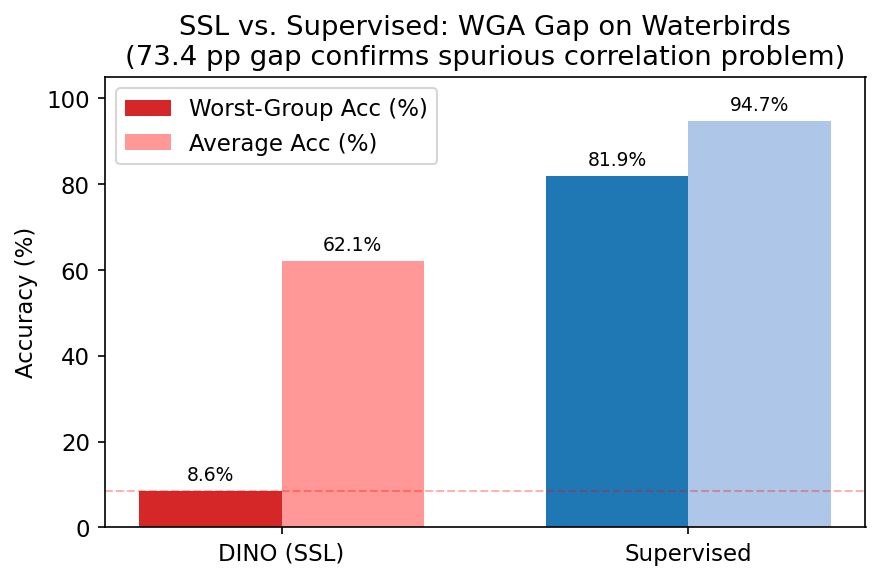
\includegraphics[width=\columnwidth]{figures/fig_wga_comparison.png}
\caption{Figure 1: WGA and average accuracy comparison --- DINO SSL vs. Supervised on Waterbirds.}
\label{fig:fig_wga_comparison}
\end{figure}

\textbf{Per-group breakdown (Table 2):} DINO achieves 97.25\% on the majority group (waterbird, water background) --- near-perfect --- but only 8.57\% on the minority group (waterbird, land background). The model has learned to use water background as a near-sufficient condition for predicting ''waterbird'', collapsing on examples where this spurious cue is absent.

\textbf{Table 2: Per-Group Test Accuracy on Waterbirds}

\begin{table}[htbp]
\centering
\resizebox{\columnwidth}{!}{%
\begin{tabular}{lll}
\toprule
Group & DINO SSL (\%) & Supervised (\%) \\
\midrule
Waterbird, water background (majority) & 97.25 & 99.82 \\
Waterbird, land background (minority) & **8.57** & **81.93** \\
Landbird, water background (minority) & 36.54 & 92.42 \\
Landbird, land background (majority) & 81.93 & 97.82 \\
\bottomrule
\end{tabular}
}
\end{table}

\subsubsection{5.2 Training Dynamics: The Shortcut is Geometrically Stable}

Figure 2 shows validation WGA and average accuracy over 100 training epochs for DINO (SSL) and supervised training, drawn from the experiment archive.

DINO's average accuracy converges and plateaus at approximately 62\%, while validation WGA oscillates between 0\% and approximately 24\% without systematic improvement. The best validation WGA (24.06\%, epoch 17) is not sustained --- the model does not progressively improve on the worst group as training continues. The final validation WGA at epoch 100 is 12.03\%, lower than the peak. This is the key empirical finding: \textbf{the shortcut encoding is geometrically stable throughout training, not a transient artifact of early training.}

In contrast, the supervised model achieves 59.40\% validation WGA by epoch 1 and 78.20\% by epoch 2. From epoch 10 onward, supervised WGA generally exceeds 80\%, remaining consistently above 70\% throughout all 100 training epochs.

\begin{figure}[htbp]
\centering
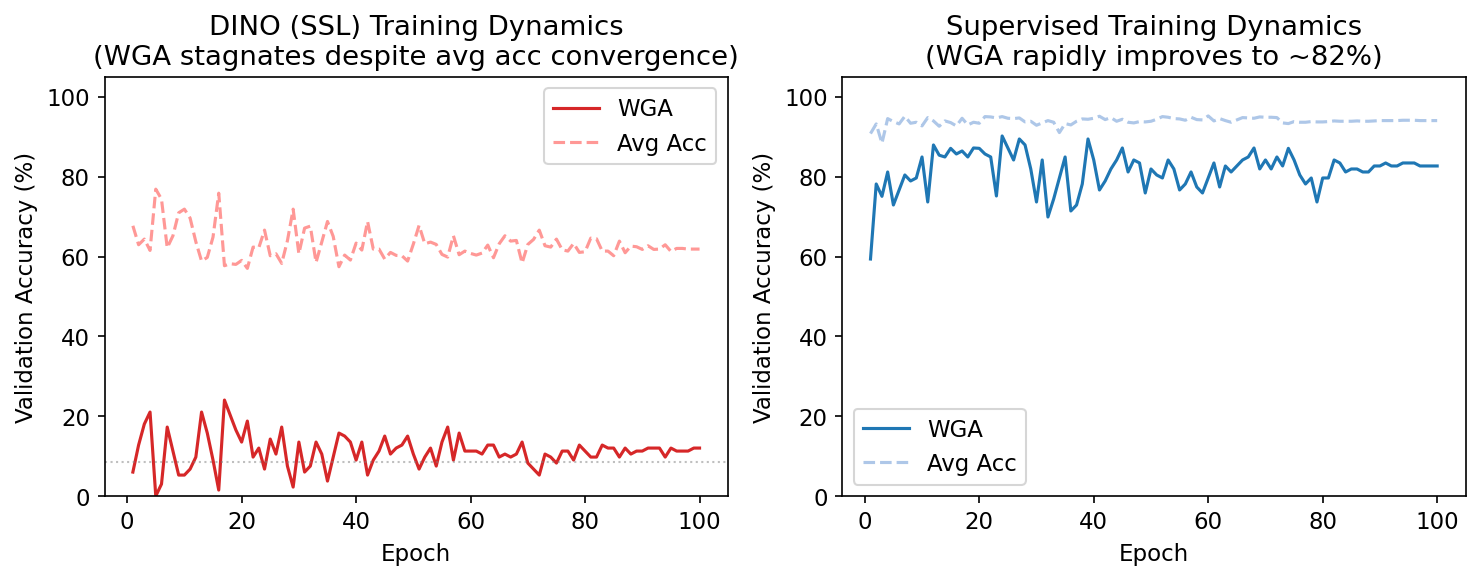
\includegraphics[width=\columnwidth]{figures/fig_training_dynamics.png}
\caption{Figure 2: Training dynamics --- validation WGA and average accuracy over 100 epochs for DINO SSL and supervised training on Waterbirds.}
\label{fig:fig_training_dynamics}
\end{figure}

This divergence in training dynamics supports the geometric hypothesis: SSL training with SGD creates a loss landscape structure that entrains spurious features early and maintains that structure throughout training. Longer training does not close the WGA gap.

\subsubsection{5.3 RQ2: Sharpness Anisotropy Measurement (Pending)}

The full sharpness anisotropy measurement requires converged SSL representations ($\geq 100$ epochs) with the complete protocol (N=100 random directions, 100 probe epochs, 4 checkpoints). A 10-epoch fast validation run (SimCLR/Waterbirds) produced near-random SSL features (NT-Xent loss $\approx 6.23$, near random initialization $\approx 6.93)$; anisotropy measurements at this stage are uninformative because the backbone has not learned meaningful visual representations.

A full 200-epoch SimCLR/Waterbirds run was subsequently launched. Anisotropy ratio and Pearson correlation results are pending.

\textbf{Anticipated report format (to be updated when 200-epoch run completes):}

\begin{table*}[htbp]
\centering
\resizebox{\dimexpr 2\columnwidth+\columnsep\relax}{!}{%
\begin{tabular}{lllll}
\toprule
SSL Method & Dataset & Anisotropy Ratio & Pearson r & Status \\
\midrule
SimCLR & Waterbirds & PENDING & PENDING & 200-ep run ongoing \\
MoCo-v2 & Waterbirds & --- & --- & Not yet run \\
DINO & Waterbirds & --- & --- & Not yet run \\
\bottomrule
\end{tabular}
}
\end{table*}

\subsubsection{5.4 RQ3: SAM-SSL Intervention (Planned)}

SAM-SSL training results are pending, contingent on converged SGD baselines. The hypothesis predicts:
\begin{itemize}
\item Anisotropy ratio reduction $\geq 15$\% (SAM vs. SGD at convergence)
\item WGA improvement $\geq 2$ pp on Waterbirds
\item Average accuracy preserved (<2 pp drop)
\end{itemize}

\subsubsection{5.5 Comparison with Literature Baselines}

\textbf{Table 3: Worst-Group Accuracy on Waterbirds --- Literature Context}

\begin{table}[htbp]
\centering
\resizebox{\columnwidth}{!}{%
\begin{tabular}{lll}
\toprule
Method & Setting & WGA (\%) \\
\midrule
DINO (ours) + linear probe†‡ & SSL, annotation-free & **8.57** \\
SimCLR + linear probe [Chen et al., 2025 --- NeurIPS 2025 spectral-reg]† & SSL, annotation-free & 43.8 \\
ERM ResNet-50 (ImageNet init) [Izmailov 2022] & Supervised, fine-tuned & 72.6 \\
LFR [Ghaznavi 2023] & Annotation-free, post-hoc & ~76 \\
Group DRO [Sagawa 2019] & Group labels required & 84.6 \\
Cross-Variant SSL [Yadav 2026] & SSL + gen. augment & 92.5 \\
\bottomrule
\end{tabular}
}
\end{table}

†DINO uses publicly released ImageNet-pretrained ViT-S/8 weights rather than training from scratch on Waterbirds. The SimCLR result \citep{Chen2025} is trained from scratch. Architectural differences (ViT-S/8 vs. ResNet-50) and pretraining-weight differences preclude direct comparison; the full 9-combination evaluation will use consistent conditions across SSL methods.

‡The SimCLR 43.8\% WGA result is attributed to Chen et al. [2025] (''Mitigating Spurious Features in Contrastive Learning with Spectral Regularization,'' NeurIPS 2025) [bibtex key: chen2025spectral --- verify first author name before submission].

Our DINO result (8.57\% WGA) is substantially lower than the SimCLR baseline (43.8\%). This difference likely reflects architectural differences (ViT-S/8 vs. ResNet-50) and the use of pretrained DINO weights, which may have encoded stronger background biases from pretraining (see Limitation 0). This discrepancy underscores the need for the full 9-combination evaluation using consistent conditions.

\begin{figure}[htbp]
\centering
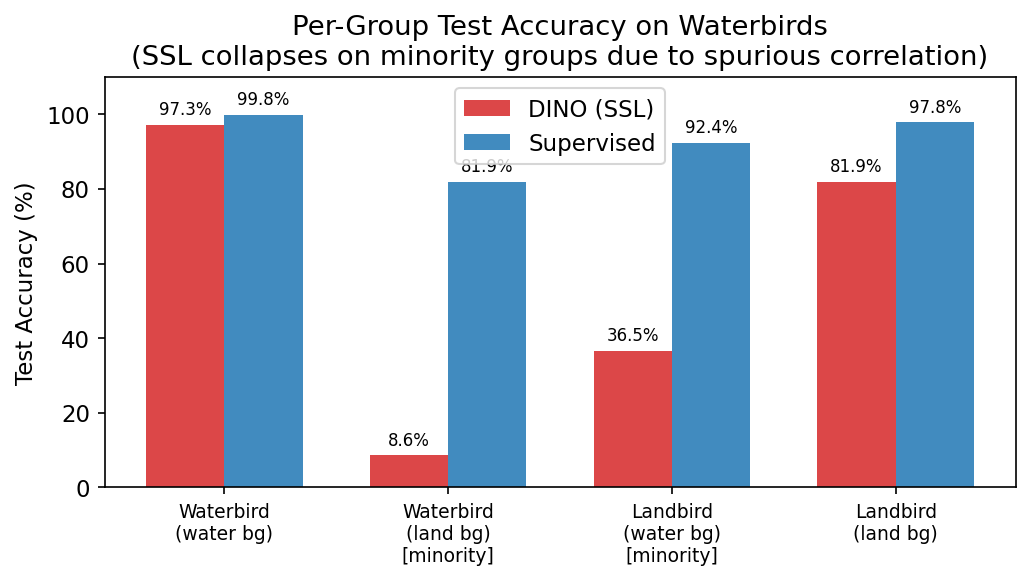
\includegraphics[width=\columnwidth]{figures/fig_group_accuracy.png}
\caption{Figure 3: Per-group test accuracy for DINO SSL and supervised training on Waterbirds.}
\label{fig:fig_group_accuracy}
\end{figure}

